\chapter{強度曲げ試験}
簡易的ではあるが.平面フレームと立体フレームの強度曲げ試験を行った.

\section{試験方法}
試験方法としてアーム中央部の根元を固定し,モータ取り付け部の先端部分に,ペットボトル容器に水を入れた重さの違うおもりをつるし,たわみ量を計測した,5N以上かけた場合,は破損してしまう可能性がったため平面フレームは5Nまでの試験とした.立体フレームは引き続き行い,33Nまで順に荷重をかけた..

\begin{figure}[htbp]
  \begin{center}
    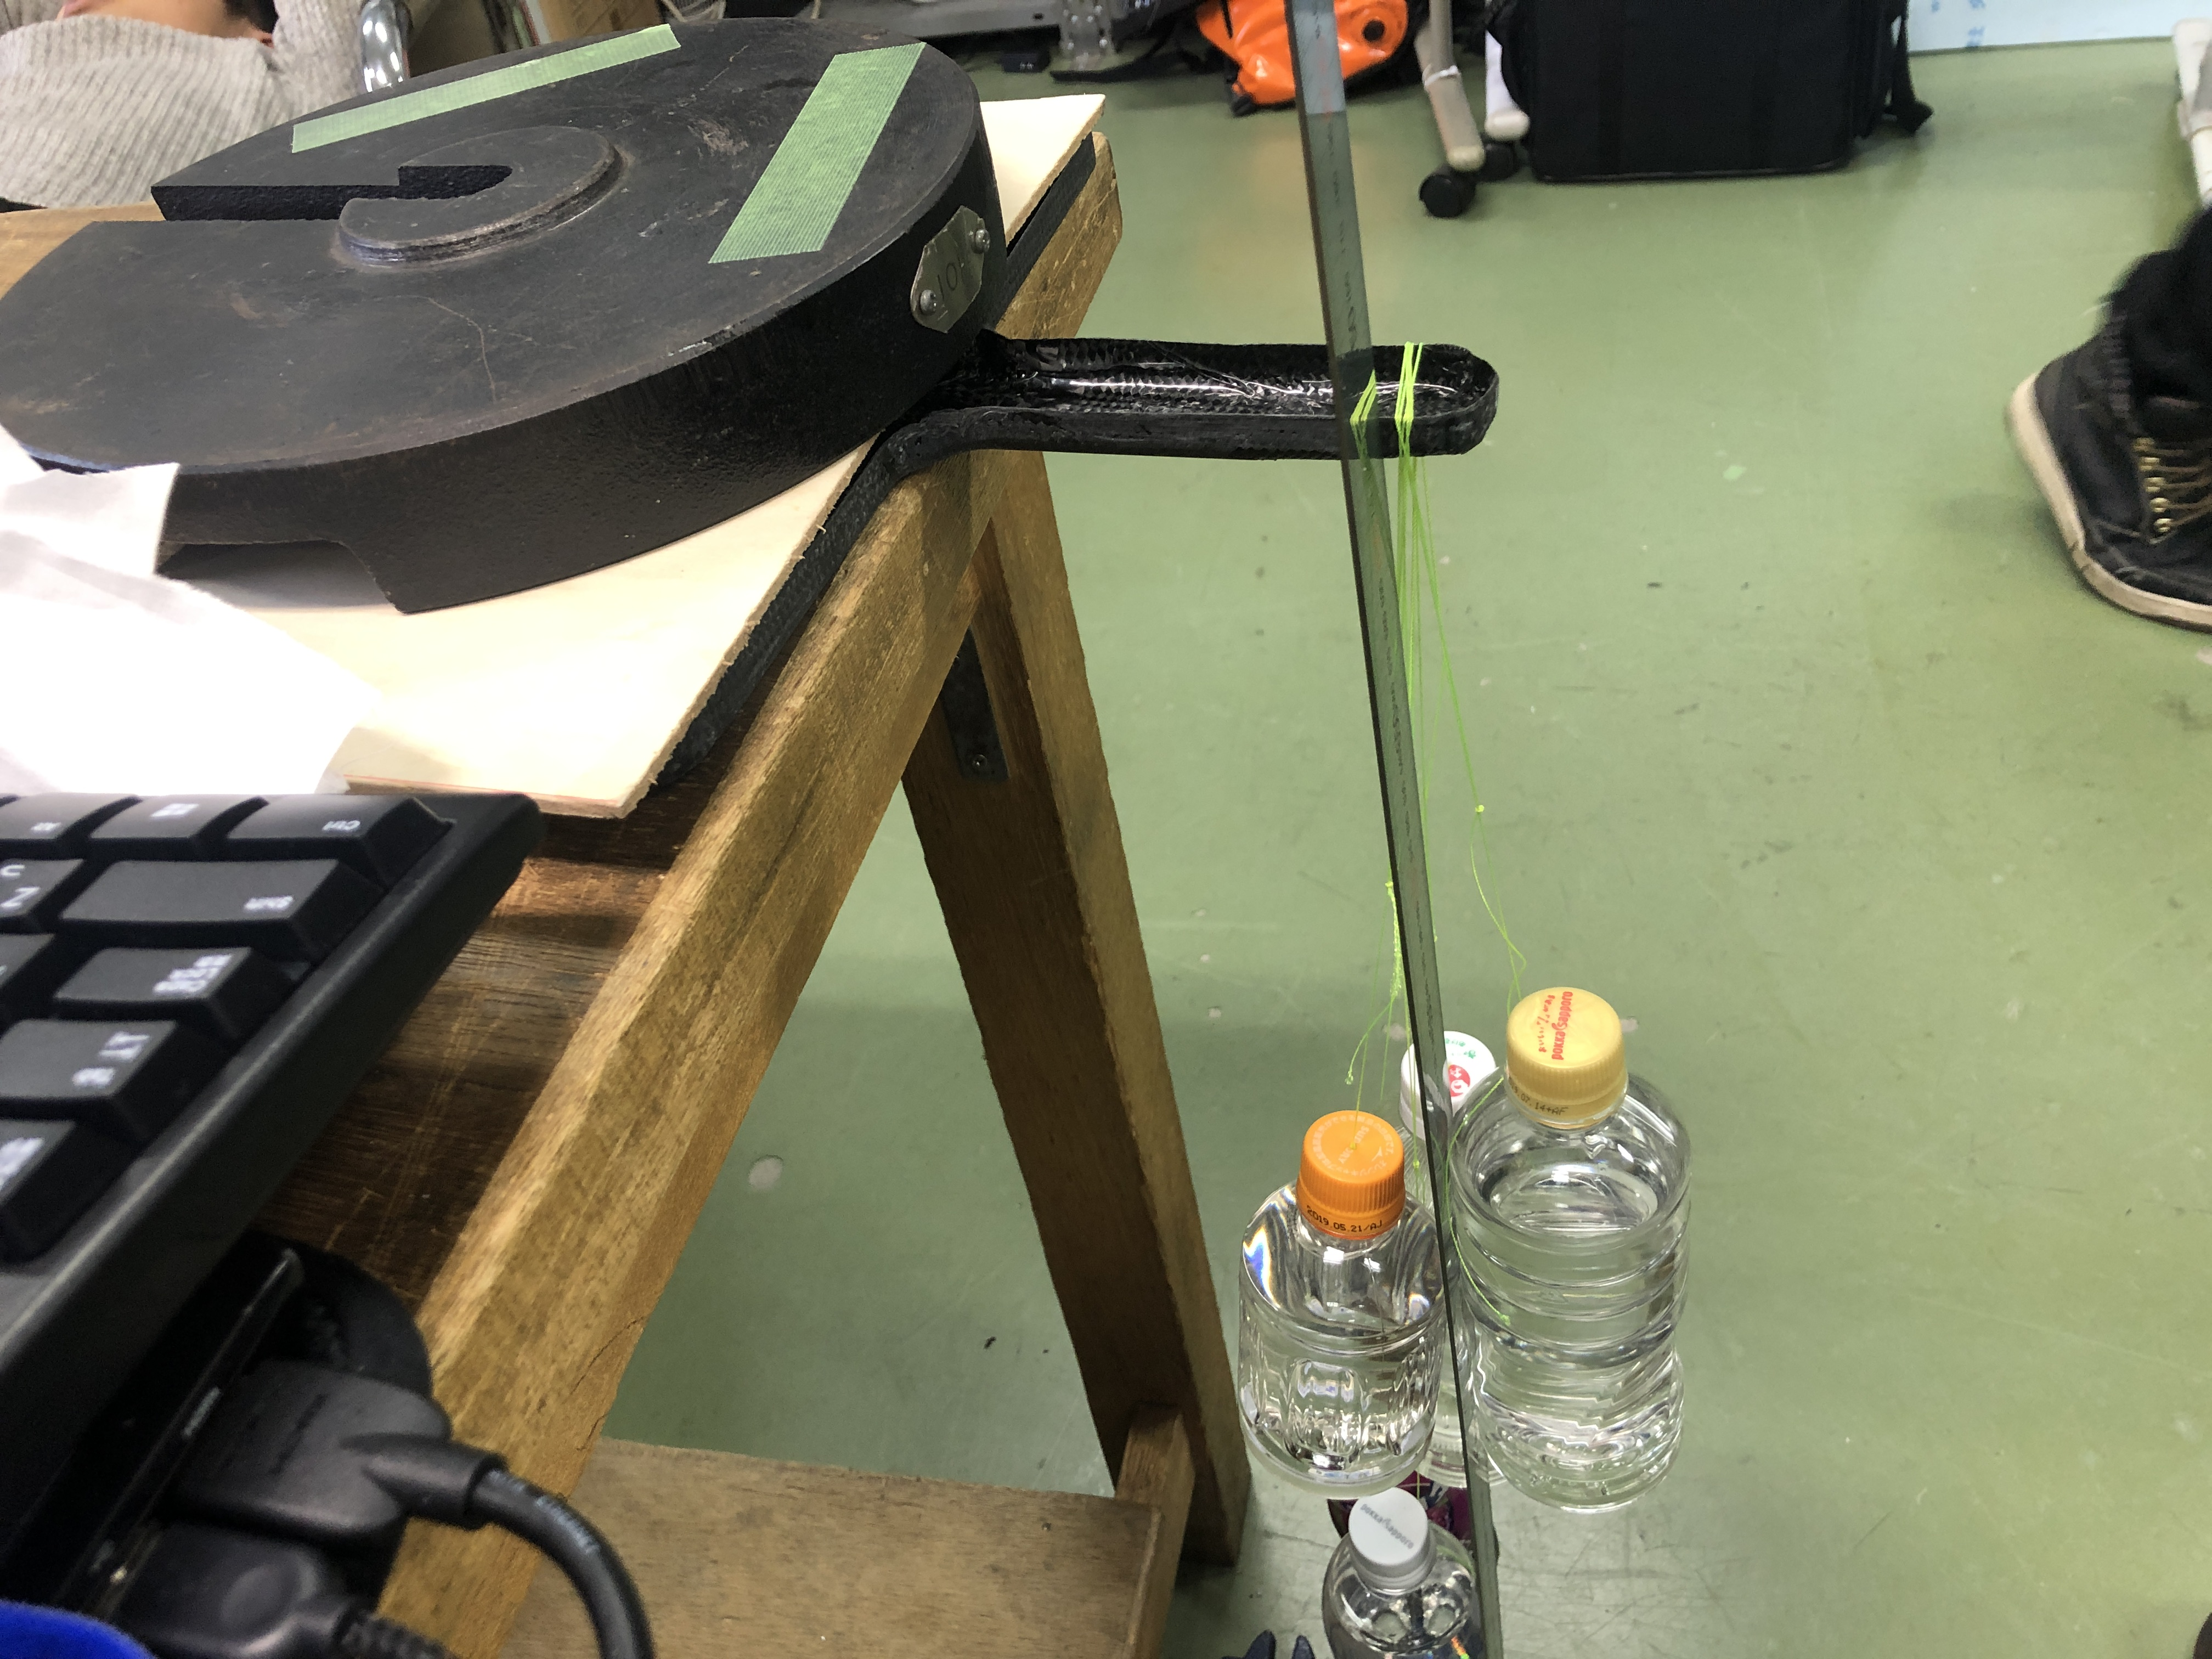
\includegraphics[width=120mm]{img/23.JPG}
    \end{center}
  \caption{おもりをつるした立体フレーム}
 \label{fig:robot}
\end{figure}

\section{試験結果}
図に示すグラフのように,平面フレームに比べ立体フレームの方が剛性が高いことがわかる.荷重が3N掛かった際に,たわみが9mmの平面フレームに対し,立体フレームは3mmである.また,5Nが掛かった際にはたわみが大幅に大きくなり平面フレームは24mm変形する.33Nの荷重がかかった立体フレームは13mm変形した.

\begin{figure}[htbp]
  \begin{center}
    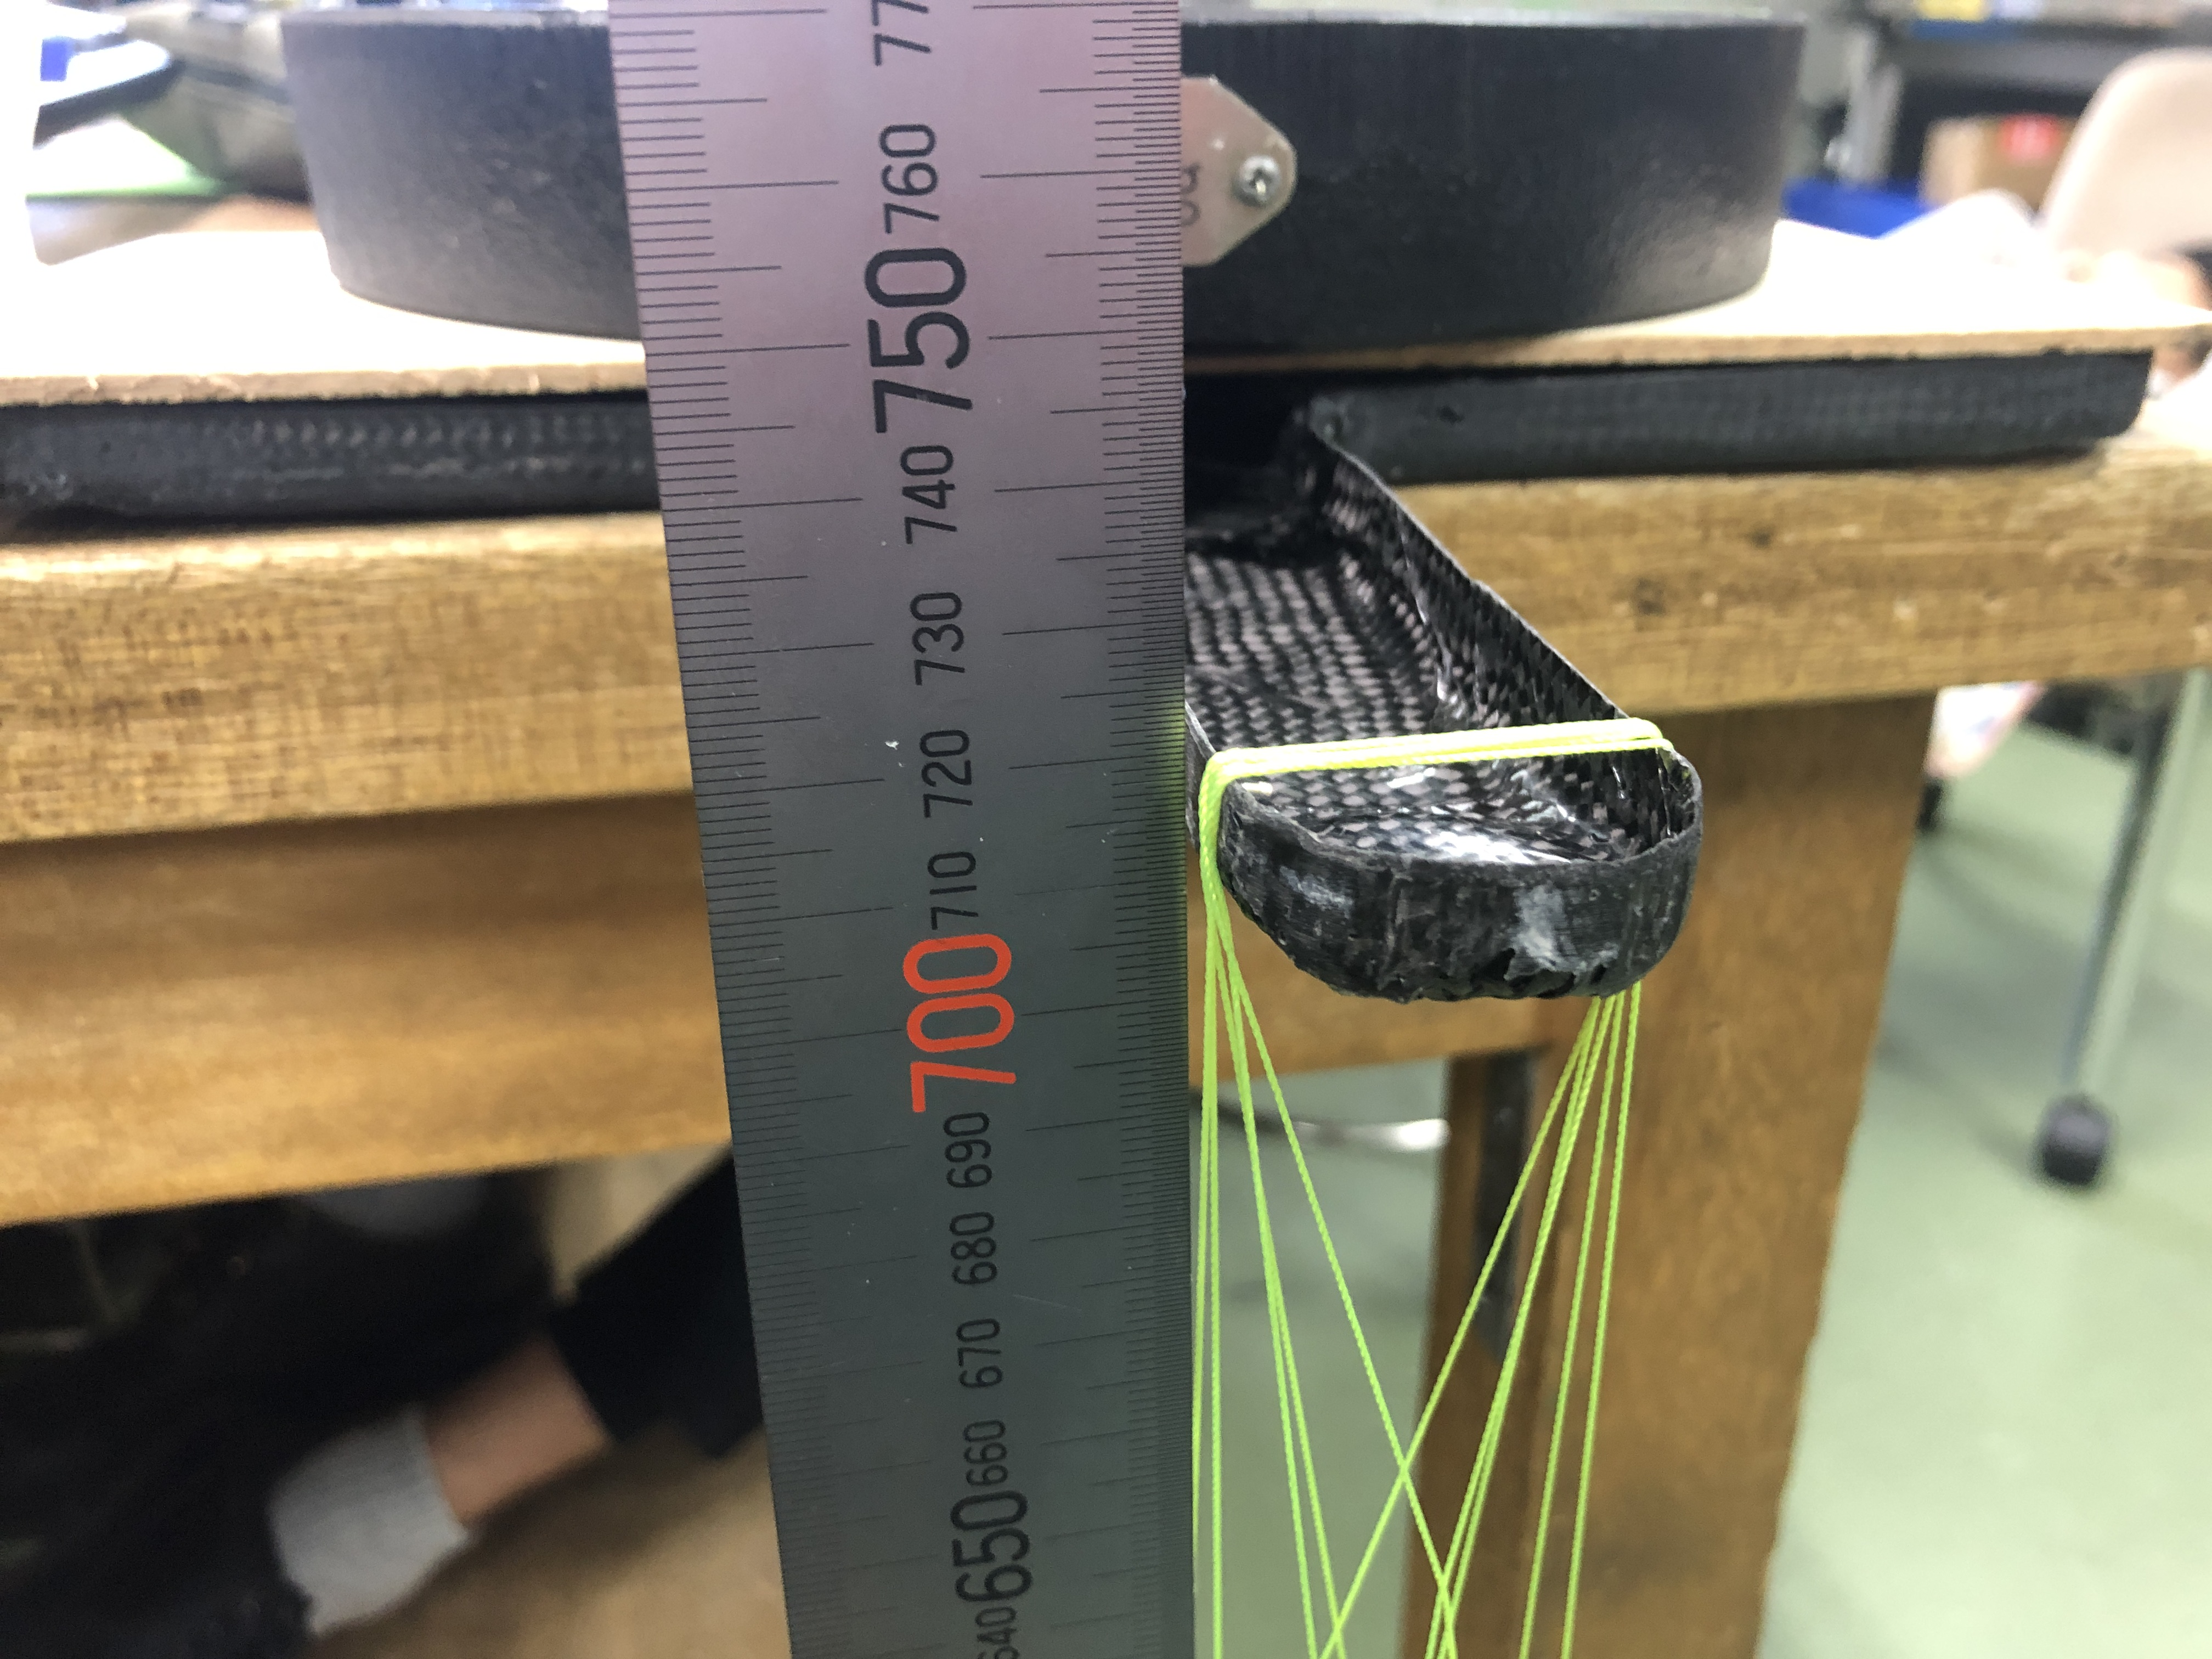
\includegraphics[width=120mm]{img/29.JPG}
    \end{center}
  \caption{たわみを計測しているフレーム}
 \label{fig:robot}
\end{figure}

\begin{figure}[htbp]
  \begin{center}
    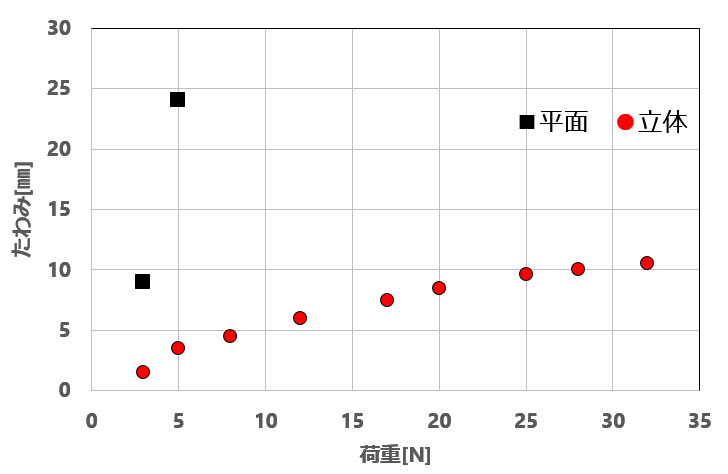
\includegraphics[width=120mm]{img/22.png}
    \end{center}
  \caption{荷重・たわみ線図}
 \label{fig:robot}
\end{figure}

\section{考察}
平面フレームから立体フレームにすることで,断面二次モーメントの値が変化する.構造物の耐久性を向上させる上で,設計上の指標として用いられる.試験結果より平面体に比べ立体の方が,断面二次モーメントが大きいため剛性が向上する.